\documentclass[crop=false, class=book]{standalone}


\usepackage{graphicx}
\usepackage[italian]{varioref}
\usepackage{copyrightbox}



\begin{document}
	\chapter{Augmented Images}
	
	
	Le API Augmented Images in ARCore consentono di rilevare e poi manipolare le immagini presenti nel mondo reale e integrarle con elementi del mondo virtuale.
	
	Dopo aver fornito delle immagini, ARCore con un algoritmo che estrae dei punti caratteristici in scala di grigi dall’immagine, ripone tutti questi dettagli in uno o più database.
	
	Durante l’esecuzione, ARCore cerca questi punti nell’ambiente consentendo di rilevare la posizione, l’orientamento e la dimensione dell’immagine nello spazio.
\begin{figure}[htp]
\centering
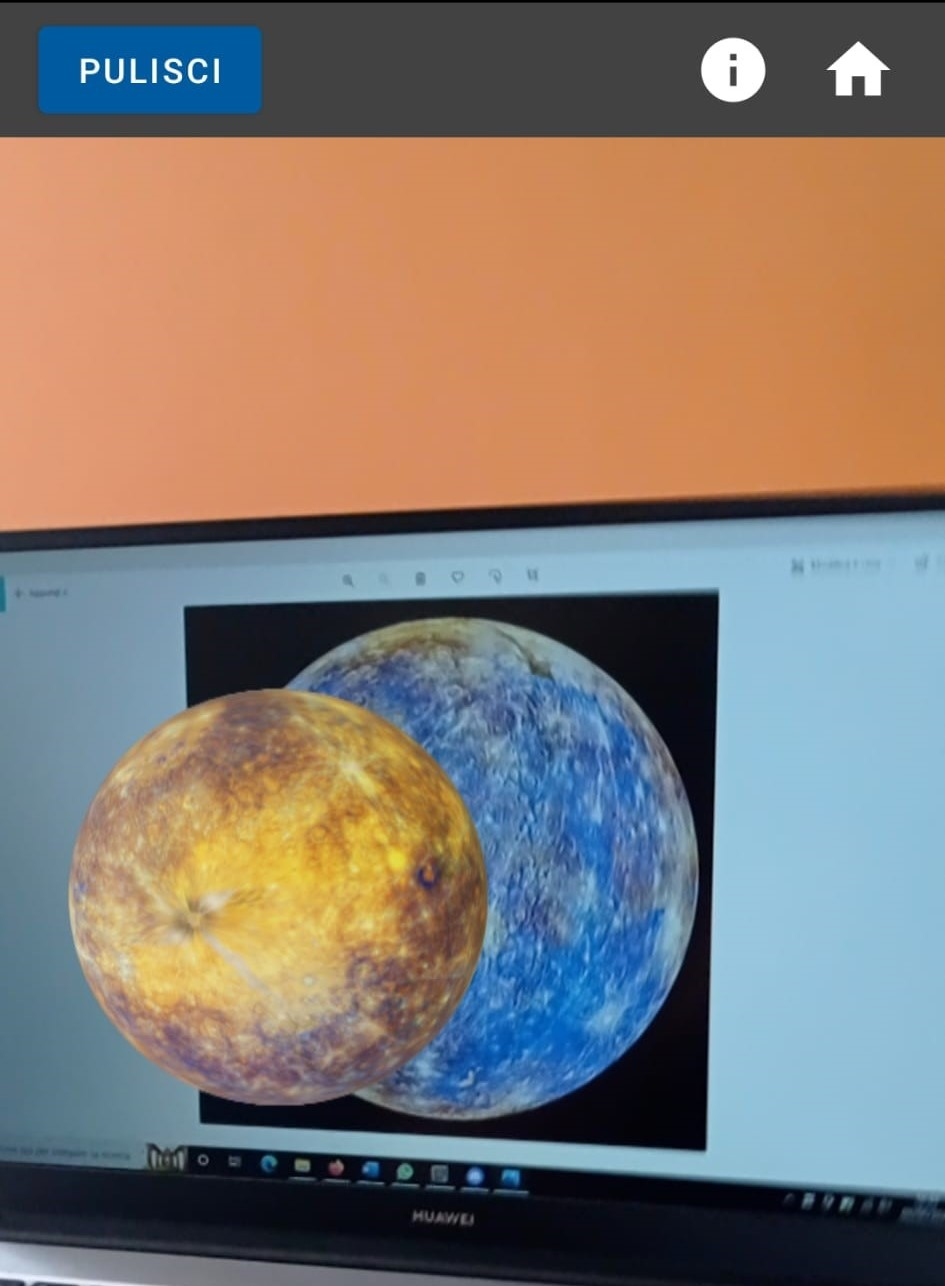
\includegraphics[width=0.5\textwidth]{./resources/images/AugmentedImages/Img1.jpeg}
\caption{Versione in 3D di mercurio} 
\end{figure}

	\section{Capacità}
	ARCore riesce a individuare fino a 20 immagini in contemporanea e non individua due istanze della stessa immagine.
	
	Il suo database riesce a contenere fino a 1000 immagini ed inoltre, non c’è limite al numero di database che possono essere caricati. L’unico vincolo è che si può attivare ed usare un singolo database alla volta.
	
	Quando si aggiunge un’immagine è possibile indicargli la sua grandezza nell’ambiente così da velocizzare il processo di tracciamento.
	
	Se non viene fornita la dimensione dell’immagine, ARCore stimerà la sua grandezza e la migliorerà durante l’esecuzione. Se viene fornita la sua dimensione ARCore ignorerà la discrepanza tra la dimensione attuale e quella segnalata e scalerà tutto secondo la dimensione dell’immagine dichiarata.
	
	ARCore è in grado di rilevare e tracciare sia immagini fisse, come ad esempio un poster nel muro, oppure immagini in movimento, come ad esempio un utente che ha l’immagine nella sua mano.
	
	Una volta che l’immagine viene rilevata ARCore continua ad ottenere informazioni ed a rifinire la sua stima dell’immagine nell’ambiente (\verb|FULL_TRACKING|).
	
	Se l’immagine si muove fuori dall’inquadratura ARCore continua a stimare la sua posizione assumendo che l’immagine sia statica e non si muova nell’ambiente (\verb|LAST_KNOWN_POSE|).

	
	\section{Requisiti}
	L’immagine deve:
	\begin{itemize}
		\item Essere visibile almeno al 25\% nell'inquadratura
		\item Essere piatta e non accartocciata
		\item Essere libera da ogni oggetto tra la fotocamera e l'immagine. Non deve essere oscurata, vista troppo angolata oppure vista quando la fotocamera si muove troppo velocemente
	\end{itemize}

	
	\section{Utilizzo della CPU e considerazioni sulle performance}
	
	In base alle funzionalità di ARCore abilitate, la batteria potrebbe scaricarsi più velocemente e può aumentare l’utilizzo della CPU. E’ consigliato disabilitare le funzionalità non utilizzate per preservare la batteria e rendere più leggero il carico della CPU.
	
	\section{Creazione del database}
	Esistono due metodi per creare un database di immagini che verranno successivamente usate da ARCore.
	
	Il primo metodo è importare un database creato in precedenza con il tool \textit{arcoreimg}.
	Per importarlo si procede come descritto dal listing~\vref{lst:ai_dbimport}, tratto dalla guida ufficiale.
	
	\begin{center}
		\begin{minipage}{0.95\textwidth}
		\begin{lstlisting}[caption={Importazione database.}, label={lst:ai_dbimport}, language=Kotlin]
		 val imageDatabase = this.assets.open("example.imgdb").use  {
			
			 AugmentedImageDatabase.deserialize(session, it)
		 }
		\end{lstlisting}
		\end{minipage}
	\end{center}
	
	Il secondo metodo consiste nel crearlo a runtime partendo con delle immagini contenuti nella cartella assets dell’applicazione, come descritto dal listing~\vref{lst:ai_dbruntime}.
	
	\begin{center}
		\begin{minipage}{0.95\textwidth}
		\begin{lstlisting}[caption={Creazione del database.}, label={lst:ai_dbruntime}, language=Kotlin]
		 val imageDatabase = AugmentedImageDatabase(session)
		
		 val bitmap = assets.open("dog.jpg").use {  BitmapFactory.decodeStream(it) }
		
		 // If the physical size of the image is not known, use  addImage(String, Bitmap) instead, at the
		 // expense of an increased image detection time.
		
		 val imageWidthInMeters = 0.10f // 10 cm
		
		 val dogIndex = imageDatabase.addImage("dog", bitmap,  imageWidthInMeters)
		\end{lstlisting}
		\end{minipage}
	\end{center}
	
	\section{Tool arcoreimg}	
	
	Per la creazione del database non a runtime si può utilizzare il tool fornito nel SDK di Google ARCore 	per Android chiamato Arcoimg.
	
	Oltre a creare il database, questo strumento permette di calcolare quanto è adatta per essere individuata dalla libreria.
	Per valutarla bisogna usare il proprio terminale e scrivere:
	\begin{center}
	
	\begin{minipage}{0.95\textwidth}
	\begin{lstlisting}[caption={Valutazione delle immagini}, label={lst:ai_session}, language=Kotlin]
	   arcoreimg.exe eval-img --input_image_path=image.png
	  \end{lstlisting}
	\end{minipage}
	\end{center}
	
	Se si ottiene un punteggio superiore a 75 su 100 allora l'immagine è utilizzabile all'interno del database e sarà individuata facilmente.
	
	Per avere un buon punteggio bisogna che le immagini non abbiano molte ripetizioni geometriche (come i QR code). Più le immagini hanno elementi dalle forme e colori diversi, più sarà facile individuarle.
	
	
	
	\begin{center}
		\begin{figure}[htp]
			\centering
			\copyrightbox[b]{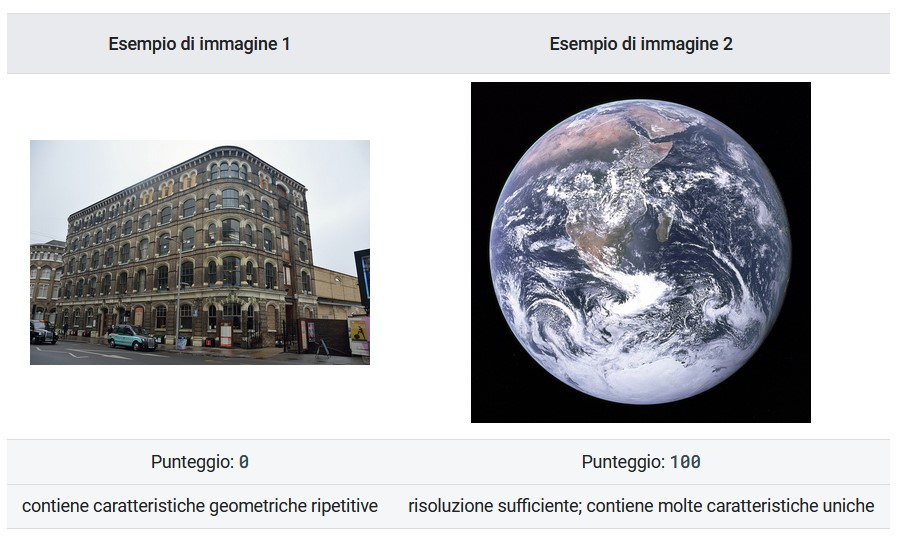
\includegraphics[width=0.9\textwidth]{./resources/images/AugmentedImages/Img2.jpg}}%
			{Fonte: \url{https://developers.google.com}}
			\caption{Esempio sulla qualità delle immagini.}
			\label{fig:env_und}
		\end{figure}
	\end{center}
	
	\section{Come abilitare il tracciamento delle immagini}
	Per abilitare il tracciamento delle immagini bisogna modificare la configurazione della sessione per impostare il database da utilizzare, come descritto dal listing~\vref{lst:ai_session}
	
	\begin{center}
		\begin{minipage}{0.95\textwidth}
		\begin{lstlisting}[caption={Descrizione del listing.}, label={lst:ai_session}, language=Kotlin]
		 val config = Config(session)
		
		 config.augmentedImageDatabase = imageDatabase
		
		 session.configure(config)
		\end{lstlisting}
		\end{minipage}
	\end{center}



\end{document}
